\chapter{Experimental Results FOR NUCLEAR SEGMENTATION PROBLEM}
\label{chap-experiment} 
\begin{ChapAbstract}
In this chapter, we describe the Hematoxylin and Eosin (H\&E) stained histopathology images dataset taken from Multi-organ Nuclei Segmentation Challenge 2018 as well as the evaluation metrics we used to evaluate our proposed methods. We also discuss more about the results acquired in each step from our algorithm, which shows the merit of each component. Moreover, the ablation study are conducted to show the improvement of our proposed enhancements.
\end{ChapAbstract}

\section{Data set and evaluation metrics}

\subsection{Hematoxylin and Eosin (H\&E) stained histopathology images dataset}

\subsubsection{Overview}
As mentioned in \cite{he_dataset_kumar}, a lot of information
about the health of the tissue to a pathologist could be revealed through histologic structure of a tissue which contributes to more general features such as shape, size, color, and crowding of glands, as well as various nuclei in epithelium and stroma. However, there are many challenges to process a whole-slide images of various type of organs as well as level of disease. "The combination of hematoxylin and eosin, or H\&E, is a ubiquitous, general,and inexpensive staining (dyeing) scheme. Hematoxylin renders nuclei dark blueish purple and epithelium light purple, while eosin renders stroma pink. Together, H\&E enhance the
contrast between nuclei, epithelium, and stroma for examination under a microscope." This dyeing scheme makes the WSIs process-able with low cost, enables the primary diagnosis. Figure \ref{fig:h_and_e_images} visualizes some examples from different organs. As mentioned, nuclear regions are enhanced by hematoxylin while pink ones are results from eosin. The contrast between nuclear and background are better after going through this dyeing scheme.

\begin{figure}[thb]
    \centering
    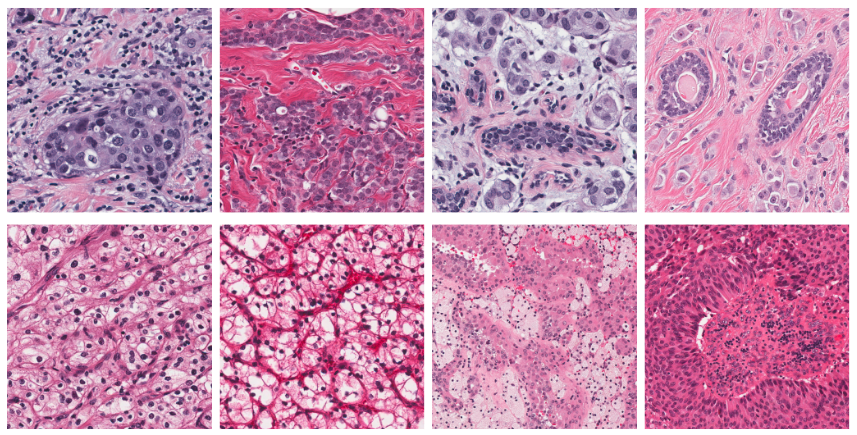
\includegraphics[width=\textwidth]{resources/5_H_E_examples.png}
    \caption{Examples of Hematoxylin and Eosin (H\&E) stained histopathology images dataset. The first row contains images from breast while the last row are from kidney.}
    \label{fig:h_and_e_images}
\end{figure}

\subsubsection{Dataset construction}
We evaluated our enhanced U-Net architecture and proposed training data augmentation approach on the data set curated by~\cite{he_dataset_kumar}, which consists of 30 histopathology images with accompanying full segmentation masks.
The images are $1000 \times 1000$ pixels in size and were extracted from WSIs from unique TCGA samples, from a variety of different organs.
To comprise the training set, four images were randomly selected from breast, liver, kidney and prostate samples. The remaining 14 images were from 7 different organs and were evenly split into validation and testing sets.

\subsubsection{Three-class ground-truth generation}

As mentioned in chapter \ref{chap-method}, we formulate nuclear segmentation as a pixel labeling problem with three potential labels, namely, nuclear interior, nuclear boundary, and background. However, there are a gap between the annotation scheme and the ground-truth we need to formalized to train our proposed network. In more details, the label provided in the dataset containing index ($id_{i,j}$) which indicates which nuclear the pixel $(i, j)$ belongs to. $id_{i,j}=0$ is the background region. We define the nuclear boundary pixel $(i,j)$ by considering ones having $id_{i,j} > 0$. If there are other pixel $(u, v)$ in a small windows which center at $(i, j)$ that $id_{u, v} > 0$ and $id_{u, v} \neq id_{i, j}$, then we consider pixel $(i, j)$ as nuclear boundary. For other cases, if $id_{i, j} = 0$, pixel $(i, j)$ is background, otherwises, it is nuclear interior. We choose windows size equals to 3. Figure \ref{fig:three_class} visualizes our defined ground-truth used to train our proposed neural network. 

\begin{figure}[thb]
    \centering
    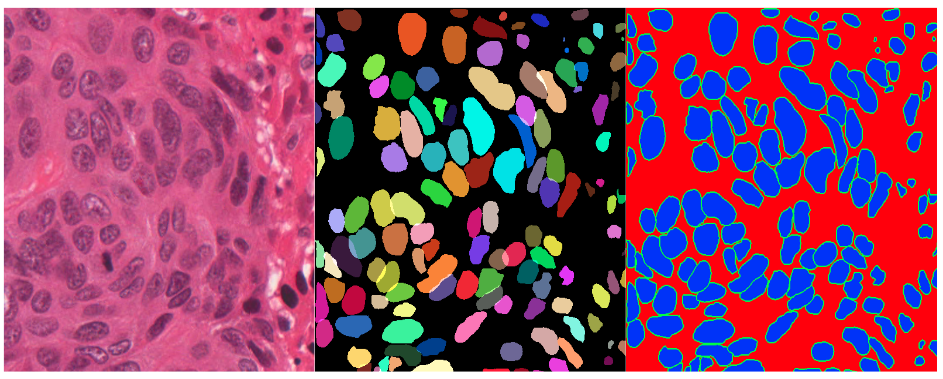
\includegraphics[width=\textwidth]{resources/5_3_classes.png}
    \caption{Proposed three-class ground-truth. The first image in input image. The middle is annotation from \cite{he_dataset_kumar}. Each color indicates different nuclear regions. The last image is the generated three-class ground-truth. Red region is background, blue is nuclear interior while green is nuclear boundary. This results are further used to train our proposed neural network.}
    \label{fig:three_class}
\end{figure}

\subsection{Evaluation metrics}

For evaluation, we focused on the AJI metric, proposed in~\cite{he_dataset_kumar}, which balances detection accuracy with the accuracy of the delineated boundaries of nuclei, though we also considered the F1-score \& Dice coefficient to shed more light upon the performance of the various architectures.

\section{Experimental setup} 
\label{sec:setup}

Our U-Net architectures operate on patches of size $128 \times 128$ (due to size limitations of the GPU), so to generate a set of training patches, we extracted random patches from each image during training.
Before extracting the patch, the original image was rotated and scaled by random amounts.
The network was trained to minimize the cross entropy loss plus the generalized Dice loss~\cite{sudre2017generalised}, which helps specifically to learn sharper boundaries by addressing the class imbalance problem of boundary pixels.
We used the Python library NiftyNet~\cite{Gibson2018} for an implementation of the Dice loss.
We adopt the weight initialization proposed in ~\cite{DBLP:journals/corr/HeZR015}.
In our experiments, we found that our enhanced U-Net works better without dropout layers, so we removed them, since they only increased the number of training steps required to converge.
We used the Adam~\cite{DBLP:journals/corr/KingmaB14} optimizer for learning.
The learning rate was set constant as $5e-5$ during the training process because of the adaptive property of Adam optimization~\cite{DBLP:journals/corr/KingmaB14}.
Our batch size was restricted to be four, due to memory limitations on the GPU.
We trained each network for roughly 300,000 steps. 
We used the validation set to fine-tune parameters.
%, including parameters for the morphological operations of the post-processing pipeline.

During test-time inference, to generate a complete segmentation map, since the images are larger than $128 \times 128$ pixels, we perform inference on overlapping patches, with an overlap of 62 pixels, and then merge the results.
We use the reflection transformation to pad patches on the boundaries of the original image.
%After feed into the network, the results of these patches are removed the added padding and placed back to the original position to assemble the mask which will go through our proposed post-processing method to create the final result.
%We used the aggregated Jaccard index (AJI) \cite{kumar2017dataset} to evaluate our model's performance.
%All of our experiments are done on TITAN V 12GB. 

\section{Experimental results}

\subsection{Synthetic dataset}
To aid in training, for each image, we generate 25 new synthetic images and their corresponding masks by our proposed method, yielding a total of 750 new synthetic images. Figure \ref{fig:new_synthetic_data} visualizes our new dataset. As can be seen in figure \ref{fig:new_synthetic_data}, there are not too much different between the original image and the synthetic one, which can improve the performance of our proposed U-Net architectures. The details are given more in section \ref{sec:ablation}.

\begin{figure}[thb]
    \centering
    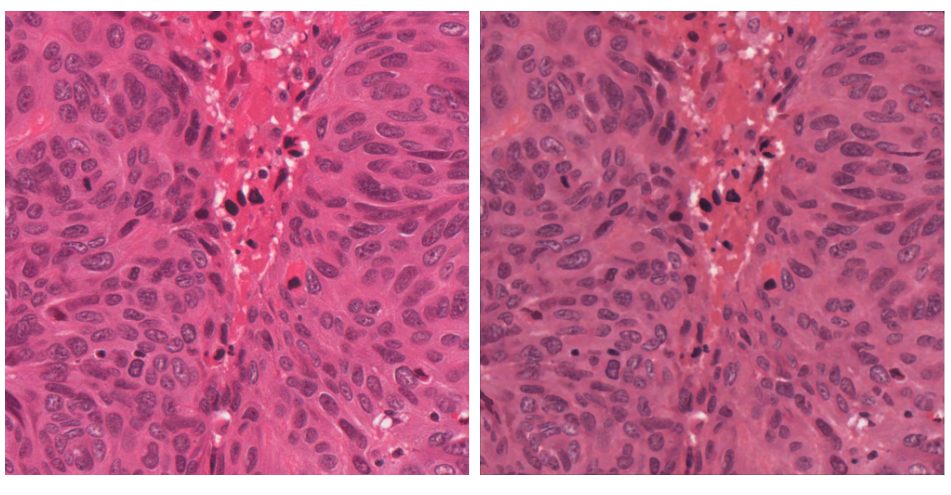
\includegraphics[width=\textwidth]{resources/5_synthetic_data.png}
    \caption{The proposed synthetic data. Left image is the original image from \cite{he_dataset_kumar} dataset, the right one is our generated image.}
    \label{fig:new_synthetic_data}
\end{figure}

\subsection{Stain normalization}

As mentioned in section \ref{chap-method}, to reduce the uninformative and possibly confusing color variation inherent to H\&E stained images, we use the structure-preserving color normalization method proposed in~\cite{7164042}. Figure \ref{fig:stain_normalize} visualizes some results from this step. The color variance in the H\&E stained histopathology images could be reduced by converting all the color space of images in dataset into same color space of a chosen one. We choose color space of image \textit{TCGA-18-5592-01Z-00-DX1} as the target space. 

\begin{figure}[thb]
    \centering
    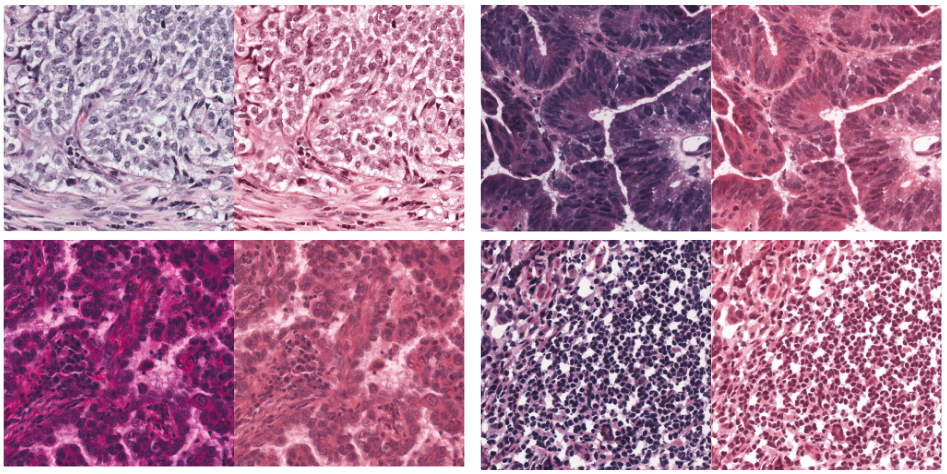
\includegraphics[width=\textwidth]{resources/5_stain_normalized.png}
    \caption{Stain normalization results. For each pair of image, the left one is the original image while the right one is the normalized image.}
    \label{fig:stain_normalize}
\end{figure}

\subsection{Post-processing results}

The results from our proposed U-Net only contain 3 class namely, nuclear interior, nuclear boundary, and background. The post-processing step is needed to assign the identify to each region in the image. Though we formalize our problem as mentioned three-class nuclear segmentation, there are much challenges to completely separate the overlapping nuclear regions. Figure \ref{fig:pose_process} visualize some of this mentioned case. With the help of post-processing step, we can alleviate this problem by applying proposed combination of morphology operations. The indexes are generated and visualized as different color in figure \ref{fig:pose_process}.

\begin{figure}[thb]
    \centering
    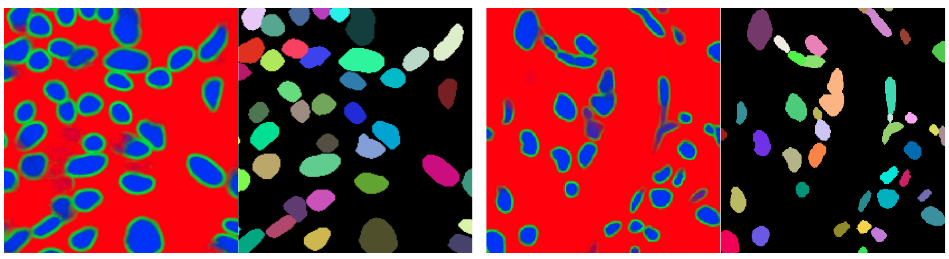
\includegraphics[width=\textwidth]{resources/5_post_processing.png}
    \caption{The U-Net results and their corresponding post-processing results.}
    \label{fig:pose_process}
\end{figure}

\subsection{Fully-enhanced network}
Fig.~\ref{fig:test_results} shows the results of our fully-enhanced U-Net, trained with augmented images, on several example histopathology images from the held-out test set, and the first row of Table~\ref{tab:ablation} shows its performance according to the aforementioned metrics.
As can be seen in Fig.~\ref{fig:test_results}, the boundary between overlapping nuclei can be reasonably separated by our method.
Moreover, our method is able to generalize well to other types of organs, even those for which it was not trained.
%As description in previous section, we only use images taken from 4 different organs including breast, liver, kidney and prostate. 
The first two lines in Fig.~\ref{fig:test_results} are from stomach and colon tissue, respectively, which tissue types were not in the training set,
yet our method still produces strong results. 
On the entire test set, our method achieved an AJI of 0.629.
For comparison, the method proposed in~\cite{he_dataset_kumar} achieved an AJI of 0.508 on the same data set, although this comparison is not definitive, since 7 fewer images from the data set were used for training in their experiments.

\begin{figure}[thb]
    \centering
    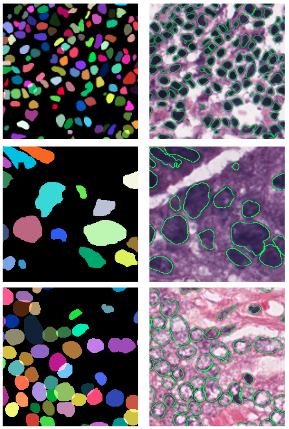
\includegraphics[width=0.85\textwidth]{resources/5_Unet_gcnn_result.png}
    \caption{Segmentation results of our fully-enhanced U-Net on example test histopathology images. \textit{Left.} Ground-truth annotations. \textit{Right.} Our results. The estimated nuclear boundary is visualized in green. Patches are cropped for better visualization. Best view in color.}
    \label{fig:test_results}
\end{figure}

%Table \ref{tab:comparison_result} shows a significant improvement of our method compared with CNN3 proposed in~\cite{kumar2017dataset}. Our method outperforms CNN3 \cite{kumar2017dataset} in all evaluation metrics. Especially, the value of AJI, which is the main metric, significantly increases by approximately 12\%. 

Processing an entire image of size $1000 \times 1000$ on a single TITAN V 12GB GPU with our enhanced U-Net architecture takes only about 17 seconds.
The subsequent post-processing incurs an additional 2 seconds on a CPU to create the final result. 

\begin{figure}[thb]
    \centering
    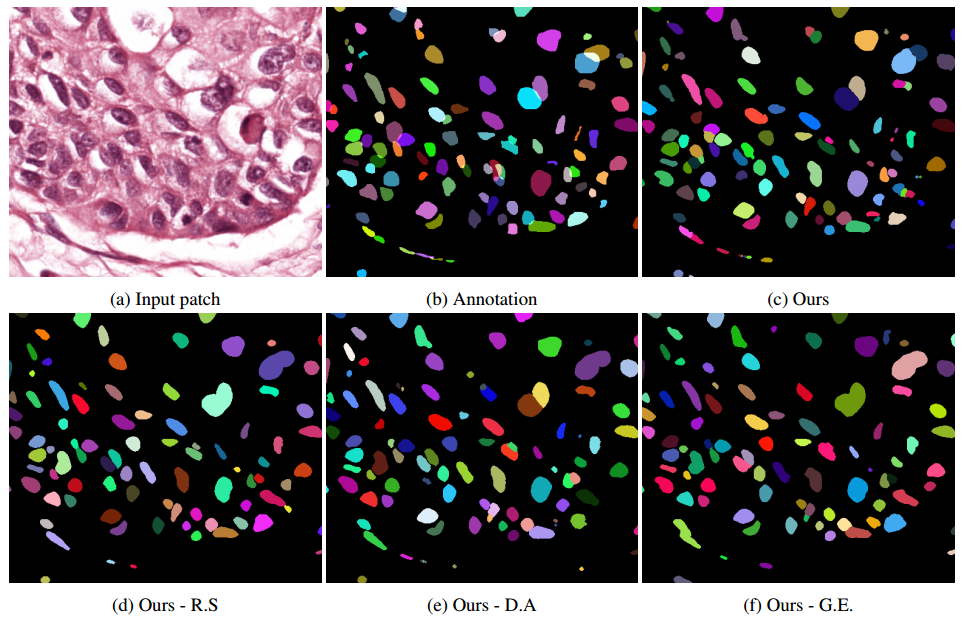
\includegraphics[width=\textwidth]{resources/5_ablation.png}
    \caption{The visualization of example results of different methods in the ablation study.
    The segmented region for each distinct detected nucleus is shown by a unique color.
    The background is visualized in black.
    Patches are cropped for better visualization.
    Best view in color.
    -D.A: without our proposed synthetic data; -R.S: without residual blocks on the long-skip connections.
-G.E.: the U-Net without group-equivariant operations.}\label{fig:vis_result}
\end{figure}

%\begin{table}
%\resizebox{0.45\textwidth}{!}{\begin{tabular}{|c|c|c|c|}
%\hline
%Method & AJI & F1-Score & Dice's Coefficient \\ \hline
%CNN3~\cite{kumar2017dataset} & 0.5083 & 0.8267 & 0.7623 \\ 
%Our method & \textbf{0.6291} & \textbf{0.8469} & \textbf{0.7980}\\
%\hline
%\end{tabular}}
%\caption{Results}
%\label{tab:comparison_result}
%\end{table}


\subsection{MoNuSeg Challenge result}

Two of three our enhancements, including new generated synthetic data and additive residual blocks along the long skip connection of U-Net architecture, are used to participate in MoNuSeg Challenge 2018. There are some differences of the solution we used to participate in this challenge. In the details, we extract patches of size $256 \times 256$ from augmented, pre-processed images for training data. For validation, we use a subset of the original images, one of each organ, leaving the other 23 images for training. Rotation and scaling are used when extracting these patches. Other configurations are kept as description in section \ref{sec:setup}. Table \ref{tab:challenge_result} shows our result in the competition. With two proposed enhancements, we rank $11^{th}$ among $32$ participants around the world, with 65.65\% as our performance.

\begin{table}[]
\centering
\begin{tabular}{|c|l|c|l|c|}
\hline
Rank        & Team                                                         & AJI             & \multicolumn{1}{c|}{Affiliation}                                                                                                                                 & Country      \\ \hline
1           & \begin{tabular}[c]{@{}c@{}}CUHK\&\\ IMSIGHT\end{tabular}     & 0.6907          & \begin{tabular}[c]{@{}l@{}}The Chinese University \\ of Hong Kong;\\ Imsight Technology\end{tabular}                                                             & China        \\ \hline
2           & BUPT.J.LI                                                    & 0.6868          & \begin{tabular}[c]{@{}l@{}}Beijing University of Post and \\ Telecommunication\end{tabular}                                                                      & China        \\ \hline
3           & pku.hzq                                                      & 0.6852          & Peking University                                                                                                                                                & China        \\ \hline
4           & Yunzhi                                                       & 0.6788          & University of Oklahoma                                                                                                                                           & USA          \\ \hline
5           & Navid Alemi                                                  & 0.6779          & University of Warwick                                                                                                                                            & UK           \\ \hline
6           & xuhuaren                                                     & 0.6642          & \begin{tabular}[c]{@{}l@{}}Shanghai Jiao Tong University\\ National University of \\ Defense Technology\end{tabular}                                             & China        \\ \hline
...         & ...                                                          & ...             & ...                                                                                                                                                              & ...          \\ \hline
\textbf{11} & \textbf{\begin{tabular}[l]{@{}c@{}}CMU-\\ UIUC-\\HCMUS\end{tabular}} & \textbf{0.6557} & \textbf{\begin{tabular}[c]{@{}l@{}}Carnegie Mellon University; \\ University of Illinois at \\ Urbana-Champaign; \\ University of Science, \\VNU-HCM\end{tabular}} & \textbf{\begin{tabular}[c]{@{}c@{}}USA\\ Vietnam\end{tabular}} \\ \hline
12          & Graham\&Vu                                                   & 0.6532          & \begin{tabular}[c]{@{}l@{}}University of Warwick, \\ Sejong University\end{tabular}                                                                              & UK           \\ \hline
13          & Unblockabulls                                                & 0.6514          & American Express, India                                                                                                                                          & India        \\ \hline
14          & \begin{tabular}[c]{@{}c@{}}Tencent \\ AI Lab\end{tabular}    & 0.6459          & \begin{tabular}[c]{@{}l@{}}University of California, Berkeley; \\ The Hong Kong University of \\ Science and Technology\end{tabular}                             & USA          \\ \hline
...         & ...                                                          & ...             & ...                                                                                                                                                              & ...          \\ \hline
29          & VISILAB                                                      & 0.4441          & \begin{tabular}[c]{@{}l@{}}Visilab Research Group, \\ University of Castilla-La Mancha, \\ Ciudad Real, Spain\end{tabular}                                       & Spain        \\ \hline
30          & Sabarinathan                                                 & 0.4437          & Cognizant Technology Solutions                                                                                                                                   & India        \\ \hline
31          & Silvers                                                      & 0.278           & Xiamen University                                                                                                                                                & China        \\ \hline
32          & TJ                                                           & 0.1301          & Tongji University                                                                                                                                                & China        \\ \hline
\end{tabular}
\caption{MoNuSeg Challenge 2018 result.}
\label{tab:challenge_result}
\end{table}

\subsection{Ablation study}
\label{sec:ablation}

We further evaluated the effect of each proposed component to the performance of our method through an ablation study. 
Example resulting segmentations from each of the following experiments are shown in Fig.~\ref{fig:vis_result} and the performance according to the aforementioned metrics are given in Table~\ref{tab:ablation}.

\begin{table}
\centering
\begin{tabular}{|c|c|c|c|c|}
\hline
Method          & AJI    & F1-score & Dice's coef. & \#Params  \\ \hline
Ours        & \textbf{0.6291} & 0.8469   & \textbf{0.7980}             & 102M      \\
Ours - D.A  & 0.6019 & 0.8006   & 0.7796             & 102M      \\
Ours - R.S  & 0.6151 & 0.8349   & 0.7846             & 101M      \\
Ours - G.E. & 0.6125 & \textbf{0.8490}   & 0.7893             & 101M \\ \hline   
\end{tabular}
\caption{Quantitative comparison of each proposed component of the U-Net architecture and training procedure.
-D.A: without our proposed synthetic data; -R.S: without residual blocks on the long-skip connections;
-G.E.: the U-Net without group-equivariant operations.}
\label{tab:ablation}
\end{table}

\subsubsection*{Residual blocks on long-skip connections}
In this experiment, we removed all residual blocks on the long-skip connections of the U-Net architecture.
To make a fair comparison, we compensated by adding more residual blocks in the encoder and decoder components to maintain the number of trainable parameters.
All of other hyper-parameters were kept constant.
The first and third line in Table~\ref{tab:ablation} show the comparison between the two different models.
Without residual blocks on the long-skip connection, the AJI value decreased by 1.4\%, and the Dice score and F1-score decreased by 1.3\% and 1.2\%, respectively.
This strengthens the credibility of our hypothesis that residual blocks on the long-skip connections help the network extract richer low-level features and thereby aid the network in delineating nuclear boundaries of touching nuclei.
Fig.~\ref{fig:vis_result}c and \ref{fig:vis_result}d further visualize the results of the two architectures.
Some nuclei in Fig.~\ref{fig:vis_result}d evidence a difficulty in separating their overlap, while our architecture with long-skip residual blocks successfully separates them. 

\subsubsection*{New synthetic data}
To see the effect of the new synthetic data we proposed, we withheld these synthetic images from the training set and trained a separate network on this reduced training set.
The architecture of the network and all of other hyper-parameters were kept the same.
As can be seen in Table~\ref{tab:ablation}, training with these new synthetic images can improve the model's performance by approximately 2.7\% in AJI, showing the most profound impact upon performance compared to the other two contributions.
This suggests that this method of data augmentation further offsets the problem of sample scarcity for histopathological analysis, even beyond standard augmentation techniques.
This is significant since labeling this type of data is extremely labor intensive.

\subsubsection*{Group equivariance}
%The purpose of including group-equivariance is to preserving equivariance to rotation transformations throughout the network, which frees a lot of parameters from the learning these transformations.
To see the effect of group-equivariant operations, we replaced these operations with standard operations for a CNN and retrained the network. 
Following the work in~\cite{gcnn}, to preserve the same number of trainable parameters, we doubled the number of filters in each convolution layer in the ordinary network, while keeping the same architecture otherwise.
This new model was trained with a similar set of hyper-parameters, except that we increased the learning rate to $1e-4$ and we were able to use a batch size of eight, since the network did not require as much storage on the GPU as the group-equivariant version.
Since there were no group-equivariant operations, we added dropout to the model to help with regularization.
As shown in Table~\ref{tab:ablation}, both the AJI and Dice's coefficient drop by a significant margin, roughly 1.7\% and 0.9\% respectively, without encoded group equivariance.
This implies that integrating group-equivariant convolution and operations into the current U-Net architecture can indeed enable the network to learn better parameters that generalize well to simple transformations, namely, translations and rotations.
Although, since it is only equivariant to rotations of 90 degrees, the network can still benefit from data augmentation of rotations of finer, arbitrary angles.



\begin{ChapAbstract}
In this chapter, we describe the results of our proposed method. Through carefully designed experiments as well as ablation study, we have shown the value of several enhancements to the standard U-Net architecture, namely, encoding rotation and translation equivariance and adding additional residual blocks, and our novel data augmentation
method for automated nuclear segmentation in histology
images.
\end{ChapAbstract}